\newpage\subsection*{\Course \ Worksheet 10 Answers}
\begin{enumerate}
    
    \item 
    \begin{enumerate}
        \item For example $f(x) = x^3+1$. 
        \item Not possible: if there is a local max at $x=2$ then the function must be concave down at $x=2$. 
        \item Possible. A sketch of such a function is below. 
        \begin{center}
			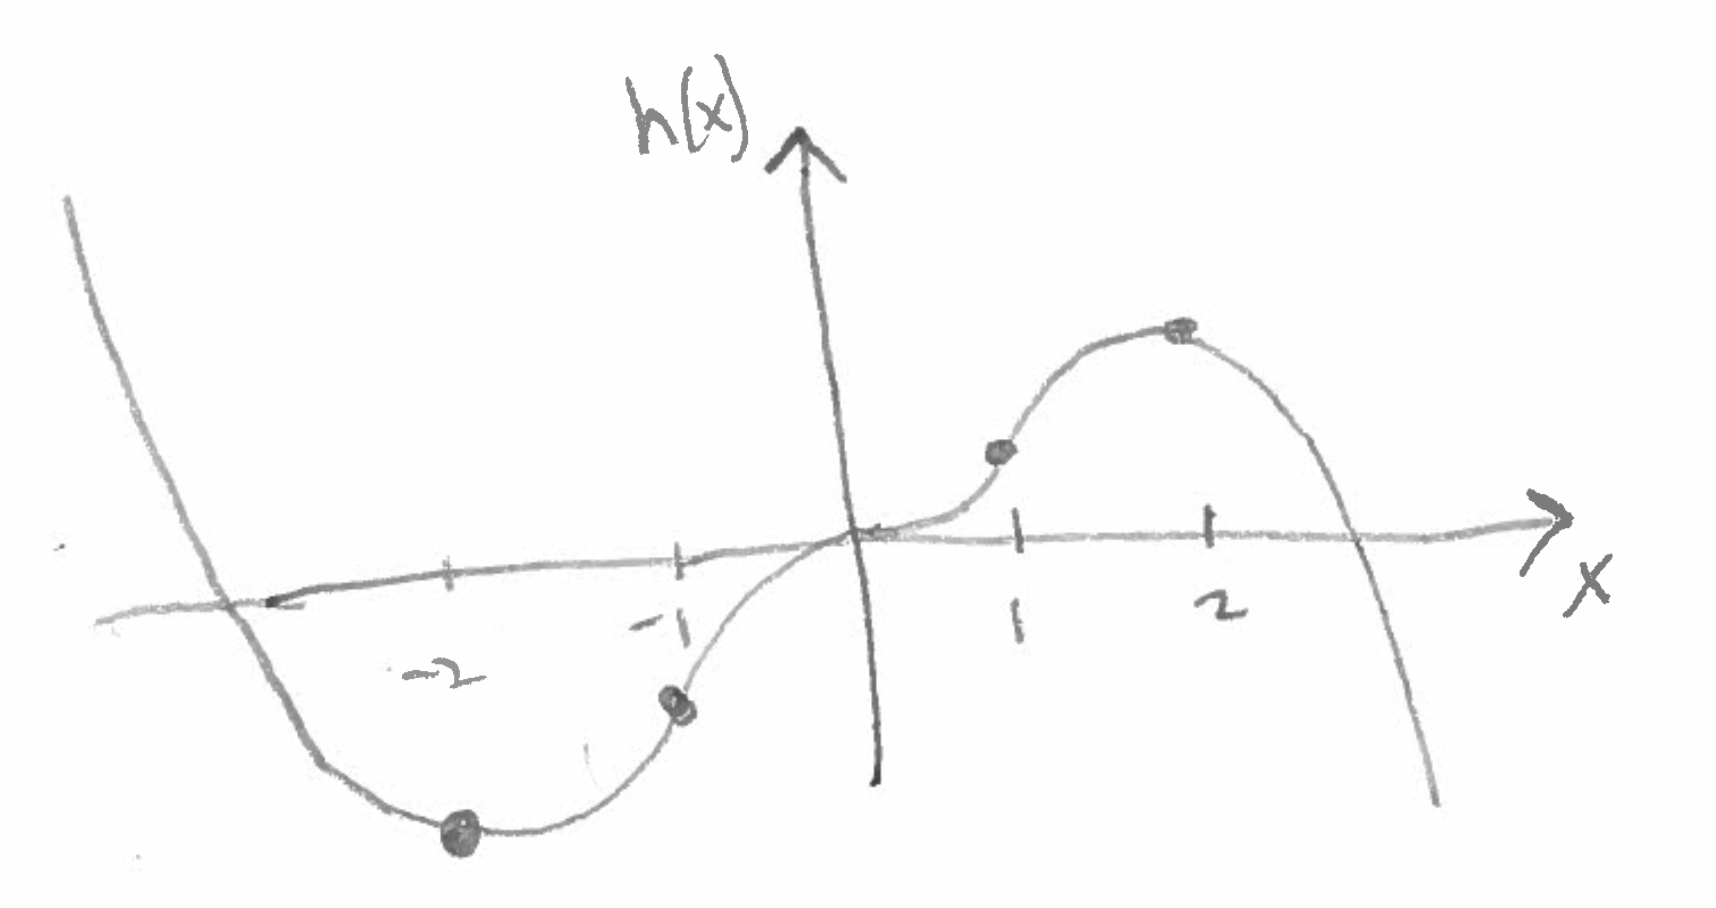
\includegraphics[width=0.8\textwidth]{images/ImgWS10Curve.png} 
		\end{center}
    \end{enumerate}
    
    \item 
        \begin{enumerate}
        \item Domain is $(-\infty,0) \bigcup (0,\infty)$
        \item Horizontal asymptote: $y\to0$ as $x\to\pm\infty$, so $y=0$ is a horizontal asymptote. \\
        Vertical asymptote: the line $x=0$ is a vertical asymptote, because $y\to\infty$ as $x\to0^+$.
        \item $y(-x) = \frac{(-x)^2 - 4}{(-x)^3} = -y(x)$, so $y$ is odd. 
        \item $x$-intercept occurs where $y=0$: 
        \begin{align*}
        	0 = \frac{x^2 - 4}{x^3} = x^2 - 4 \Rightarrow x = \pm 2
        \end{align*}
        $y$-intercepts occur where $x=0$, but $x=0$ is not in the domain, so there are no y-intercepts.
        \item Critical points occur where $y'(x) =0$. 
        \begin{align*}
        	y'(x) = 
            0 &= \ddx \left(\frac{x^2 - 4}{x^3} \right) \\ 
            0&= \ddx \left(\frac 1 x - 4x^{-3}\right) \\
            0&= -\frac{1}{x^2} + 12x^{-4} \\
            0&= -x^2 + 12 \\
            x &= \pm \sqrt{12} = \pm 2\sqrt{3}
        \end{align*}
        Thus, critical points at $x = \pm 2\sqrt{3}$. 
        
        \begin{center}
			\begin{tabular}{ c c c c c c c c}
              & $(-\infty,-2\sqrt{3})$ & $-2\sqrt{3}$ & $(-2\sqrt{3},0)$ & 0 & $(0,2\sqrt{3})$ & $2\sqrt{3}$ & $(0,\infty)$ \\ 
            \hline \vspace{2pt}
			$y'(x)$ & - & 0 & + & undefined & + & 0 & - \\  
            \vspace{2pt}
 			$y(x)$ & decreasing & min & increasing & undefined & increasing & max & decreasing\\
            \hline
		\end{tabular}
		\end{center}
        \item Inflection points occur where $y''(x) = 0$. 
        \begin{align*}
        	y''(x) =
            0 &= \ddx \left(-x^{-2} + 12x^{-4} \right) \\
            0&= 2x^{-3} - 48x^{-5}\\
            0&=  2x^2 - 48 \\
            x^2 &= 24 
        \end{align*}
        Thus, inflection points at $x = \pm 2\sqrt{6}$. IP = inflection point.
        \begin{center}
			\begin{tabular}{ c c c c c c c c}
              & $(-\infty,-2\sqrt{6})$ & $-2\sqrt{6}$ & $(-2\sqrt{6},0)$ & 0 & $(0,2\sqrt{6})$ & $2\sqrt{6}$ & $(0,\infty)$ \\ 
            \hline \vspace{2pt}
			$y''(x)$ & - & 0 & + & undefined & + & 0 & - \\  
            \vspace{2pt}
 			$y(x)$ & con. down & IP & con. up & undefined & con. down & IP & con. up\\
            \hline
		\end{tabular}
		\end{center}  
        \item Critical points are at $x = \pm 2\sqrt{3}$. By first (or second) derivative test, local min at $x = - 2\sqrt{3}$, local max at $x = 2\sqrt{3}$. There are no absolute min or max. 
        \item The function is sketched below. Don't forget to label axes. 
   
    \begin{center}
    \begin{tikzpicture}[scale=2] 
        \begin{axis}[
        clip=false,
        axis lines=middle,
        restrict y to domain=-6:6,
        axis line style={shorten >=-7.5pt, shorten <=-7.5pt},
        xlabel=$x$,
        ylabel=$y(x)$,
        xlabel style={at={(ticklabel* cs:1)},anchor=north west},
        ylabel style={at={(ticklabel* cs:1)},anchor=north east},
        arrow/.style={-stealth,DarkBlue,very thick},
        ]
        \addplot[black,samples=501,domain=0.001:12,thick] {(x*x-4)/(x*x*x)};% 
        \addplot[black,samples=501,domain=-12:-0.001,thick] {(x*x-4)/(x*x*x)};% 
        \end{axis}
    \end{tikzpicture}
    \end{center}
    
    
    
    \end{enumerate}
    
    \item Let $x$ be the length of one side of the square cut out of the sheet. 
        \begin{center}
			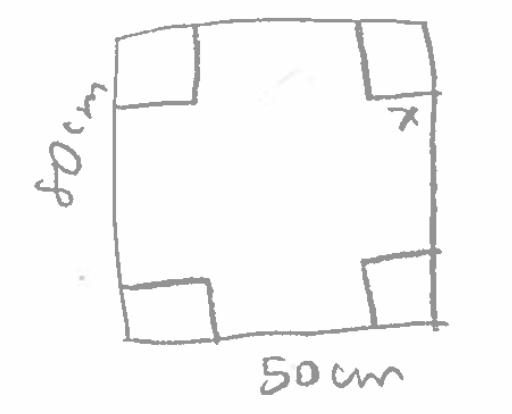
\includegraphics[width=0.4\textwidth]{images/ImgWS10Box.png} 
		\end{center}         
    Construct equation for volume, differentiate, set equal to zero, solve for $x$. 
    \begin{align*} 
    	V &= (50-2x)(80-2x) x \\
        &= 4000x-260x^2+4x^3 \\
        V'(x) &= 4000 - 520 x + 12x^2 \\
        0 &= 1000 - 130x + 3x^2 \\
        &= (3x-100) (x-10) \\
        x &= \frac{100}{3}, 10
    \end{align*}
    Volume is negative if $x=100/3$, so we set $x=10$ cm, and the volume is
        \begin{align*} 
    	V (10) &= (50-2\cdot 10)(80-2\cdot 10) 10 = 30 \cdot 60 \cdot 10 = 18,000 \ \text{cm}^3
    \end{align*}
    \item A screen capture of the solution is below.
    
    \begin{center}
			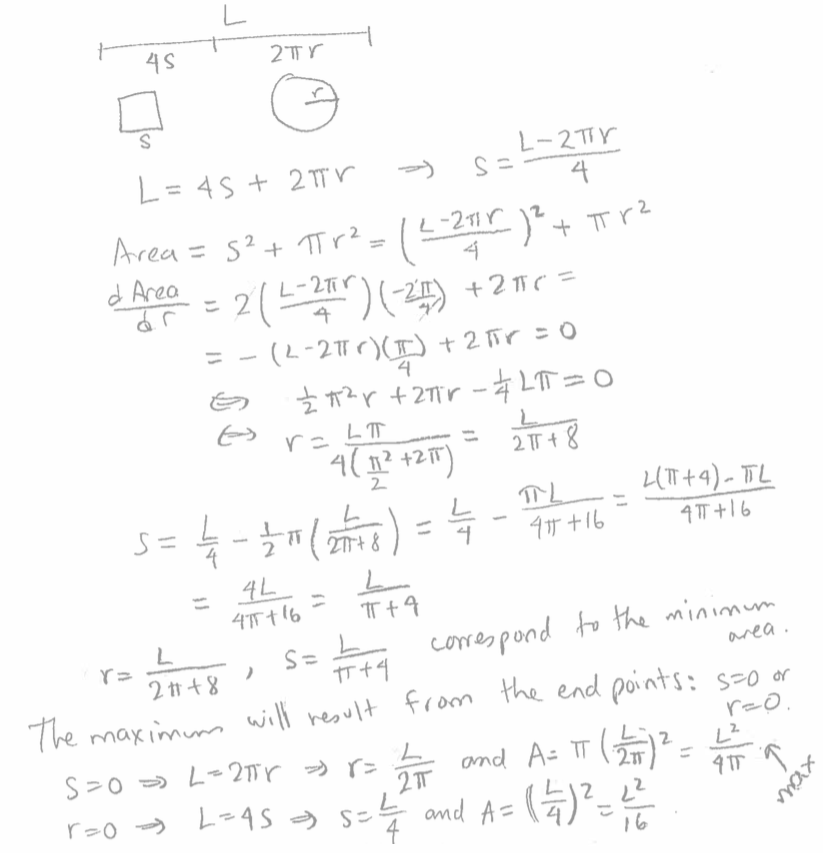
\includegraphics[width=0.8\textwidth]{images/ImgWS10Wire.png} 
	\end{center}     
\end{enumerate}
    
    
    